%%%%%%%% ICML 2021 EXAMPLE LATEX SUBMISSION FILE %%%%%%%%%%%%%%%%%

\documentclass{article}

% Recommended, but optional, packages for figures and better typesetting:
\usepackage{microtype}
\usepackage{graphicx}
\usepackage{subfigure}
\usepackage{booktabs} % for professional tables
\usepackage{multirow}
% hyperref makes hyperlinks in the resulting PDF.
% If your build breaks (sometimes temporarily if a hyperlink spans a page)
% please comment out the following usepackage line and replace
% \usepackage{icml2021} with \usepackage[nohyperref]{icml2021} above.
\usepackage{hyperref}

% Attempt to make hyperref and algorithmic work together better:
\newcommand{\theHalgorithm}{\arabic{algorithm}}

% Define the subsubsubsection command
\newcommand{\subsubsubsection}[1]{%
  \paragraph{#1}\mbox{}\\}





\usepackage[accepted]{icml2021}

\icmltitlerunning{Wine Quality Prediction}

\begin{document}

\twocolumn[
\icmltitle{Wine Quality Prediction}

\begin{icmlauthorlist}
\icmlauthor{Stijn de Preter (852726504)}{ou}
\icmlauthor{Arjan Broer (850166428)}{ou}
\end{icmlauthorlist}

\icmlaffiliation{ou}{Open Universiteit}
\icmlcorrespondingauthor{}{}

% You may provide any keywords that you
% find helpful for describing your paper; these are used to populate
% the "keywords" metadata in the PDF but will not be shown in the document
\icmlkeywords{wine quality, machine learning, neural networks, ANN, SVR }

\vskip 0.3in
]

\section{Brief Introduction}
The assignment is based on the article \cite{dahal2021prediction} and focuses on the reproduction of the article results.
The reproduct is limited to only the Support Vector Regression (SVR) and Artificial Neural Network (ANN) models.
The Ridge Regression (RR) and Gradient Boosting Regression models are not included in this report.
The goal of the assignment is to predict the quality of wine based on its chemical properties and understand the methods used to generate the predictions.
The dataset will be analyzed to find the features that most influence the quality of wine and suggestions are provided to improve the hyperparameters of the model for best results.

The research questions discussed in this report are:
\begin{enumerate}
    \item Reproduce the results of the article \cite{dahal2021prediction} using the same dataset and models.
    \item Analyze the dataset to find the features that most influence the quality of wine.
    \item Provide suggestions to improve the hyperparameters of the model for best results.
\end{enumerate}

\section{Methods}
The methods used for this assignment are based on the article \cite{dahal2021prediction} and include Support Vector Regression (SVR) and Artificial Neural Network (ANN) models.
The impact of the features is analyzed using SHAP (SHapley Additive exPlanations) values and the Pearson correlation coefficient. Improvements on the both the SVR and ANN models are investigated and reported.

\subsection{SVR and ANN - Reproduce the results}
In order to compare the results of the article with our results, a visualization was made. Here the values of the article (\textbf{still to be added}) are compared with our results repeatedly. Our results are reproduced repeatedly with different test and training data each time. This way we are sure that it is not a lucky shot but we get a realistic picture of how our model performs.
Also, standardization has been applied to the data features of the dataset, not to the quality column.

\subsection{SVR and ANN - Impact of the features}
The article analyses the impact of individual features on the quality of the wine.
This analysis is done by looking at the correlation between the features and the quality of the wine.
The correlation is calculated in the article using the Pearson correlation coefficient.
The Pearson correlation coefficient is a measure of the linear correlation between two variables.

By using SHAP (SHapley Additive exPlanations) values, the impact of the features on the model can be analyzed.
The explanation of the model should reflect a similar result as compared to the pearson correlation coefficient.
Shapley values are created by using the Shapley value method, which is a method from cooperative game theory.
Effectively it will calculate the contribution of each feature to the model output by looking at the impact of each feature on the model output.
\cite{lundberg2017unified} describes in detail how the impact of individual features is determined by retraining the model with this a feature excluded.
Then the impact of the feature on the model output is calculated by looking at the difference between the model output with and without the feature.
Diagrams used to explain the impact of features are the dependency plot and the force plot.
The dependency plot shows the impact of a feature on the model output.
The force plot shows the impact of all features on the model output.
The force plot is a more complex diagram that shows the impact of all features on the model output.

\subsection{SVR and ANN - Improve the model}
For optimizing the hyperparameters, gridsearch and BayesSearch were used for SVR. For ANN, gridsearch was used to examine the impact of the hyperparameters.


\section{Experimental Results}
This chapter, experimental results, is split into 3 parts: A short general piece, a piece on SVR and a part on ANN

\subsection{Datasets}
When exploiting the data it was found that the information given in the article about the data did not match the information about the data. The article indicates that the red wine dataset was used. Based on the number of rows and other metadata (averages, Median, ...) we see that the white wine dataset was used. In the rest of this article we will work with the white wine dataset.

\subsection{SVR}

\subsubsection{Datasets}
The article indicates that the data is split into training data and testing data with a ratio of 3:1. This is also the ratio of the splits that was applied in further research.

\subsubsection{Implementation Details}

\subsubsubsection{Reproduce the results}
The results of the article are simulated by using the parameters mentioned in the article. The following parameters are mentioned: kernel=rbf, cost = 0.95 and Gamma = 0.13. For all other parameters, the default parameters of sklearn are chosen, except for the Tolerance for stopping criterion, which is set to 0.0001 to obtain the best possible result and because the cost is negligible given the small dataset.
How the training data is chosen is unknown, so the split between training and test data is performed multiple times. In this way, there is a realistic picture of the models that generate these parameters.

\subsubsubsection{Impact of the features}
In figure \autoref{fig:dependency-plot-svr} \nameref{fig:dependency-plot-svr} the impact of the features is visualized.
The dependency plot shows the impact of each feature on the model output.
The color of the dots indicates the value of the feature, with red indicating a high value and blue indicating a low value.
The y-axis shows the impact of the feature on the model output.

The plot for alcohol shows that the impact of alcohol on the model output is positive.
This means that a higher value of alcohol leads to a higher quality of wine.
The trend of the values is clearly visible in the plot, showing a positive correlation between the feature and the model output.
This is also confirmed by the Pearson correlation coefficient, which shows a positive correlation between alcohol and quality.

The plot for density show that the impact of density on the model output is negative.
This means that a higher value of density leads to a lower quality of wine.
just as with alcohol, the trend of the values is clearly visible in the plot, showing a strong negative correlation between the feature and the model output.

The plot for chlorides shows that the impact of chlorides on the model output is also negative. Again this corresponds with the Pearson correlation coefficient, which shows a negative correlation between chlorides and quality.

THe feature with the least impact on the model output is Free sulfur dioxide.
The plot shows that the impact of Free sulfur dioxide on the model output is positive.
This means that a higher value of Free sulfur dioxide leads to a higher quality of wine.
However, the trend of the values is not clearly visible in the plot, showing a weak correlation between the feature and the model output.
This is also confirmed by the Pearson correlation coefficient, which shows a weak positive correlation between Free sulfur dioxide and quality.
Notable is that Free sulfur dioxide has a strong positive trend for the lower values. This suggests that the feature has a minumum value for the quality of wine.
This was not visible in the pearson correlation coefficient because the correlation coefficient is calculated over the entire dataset.

\begin{figure*}
    \centering
    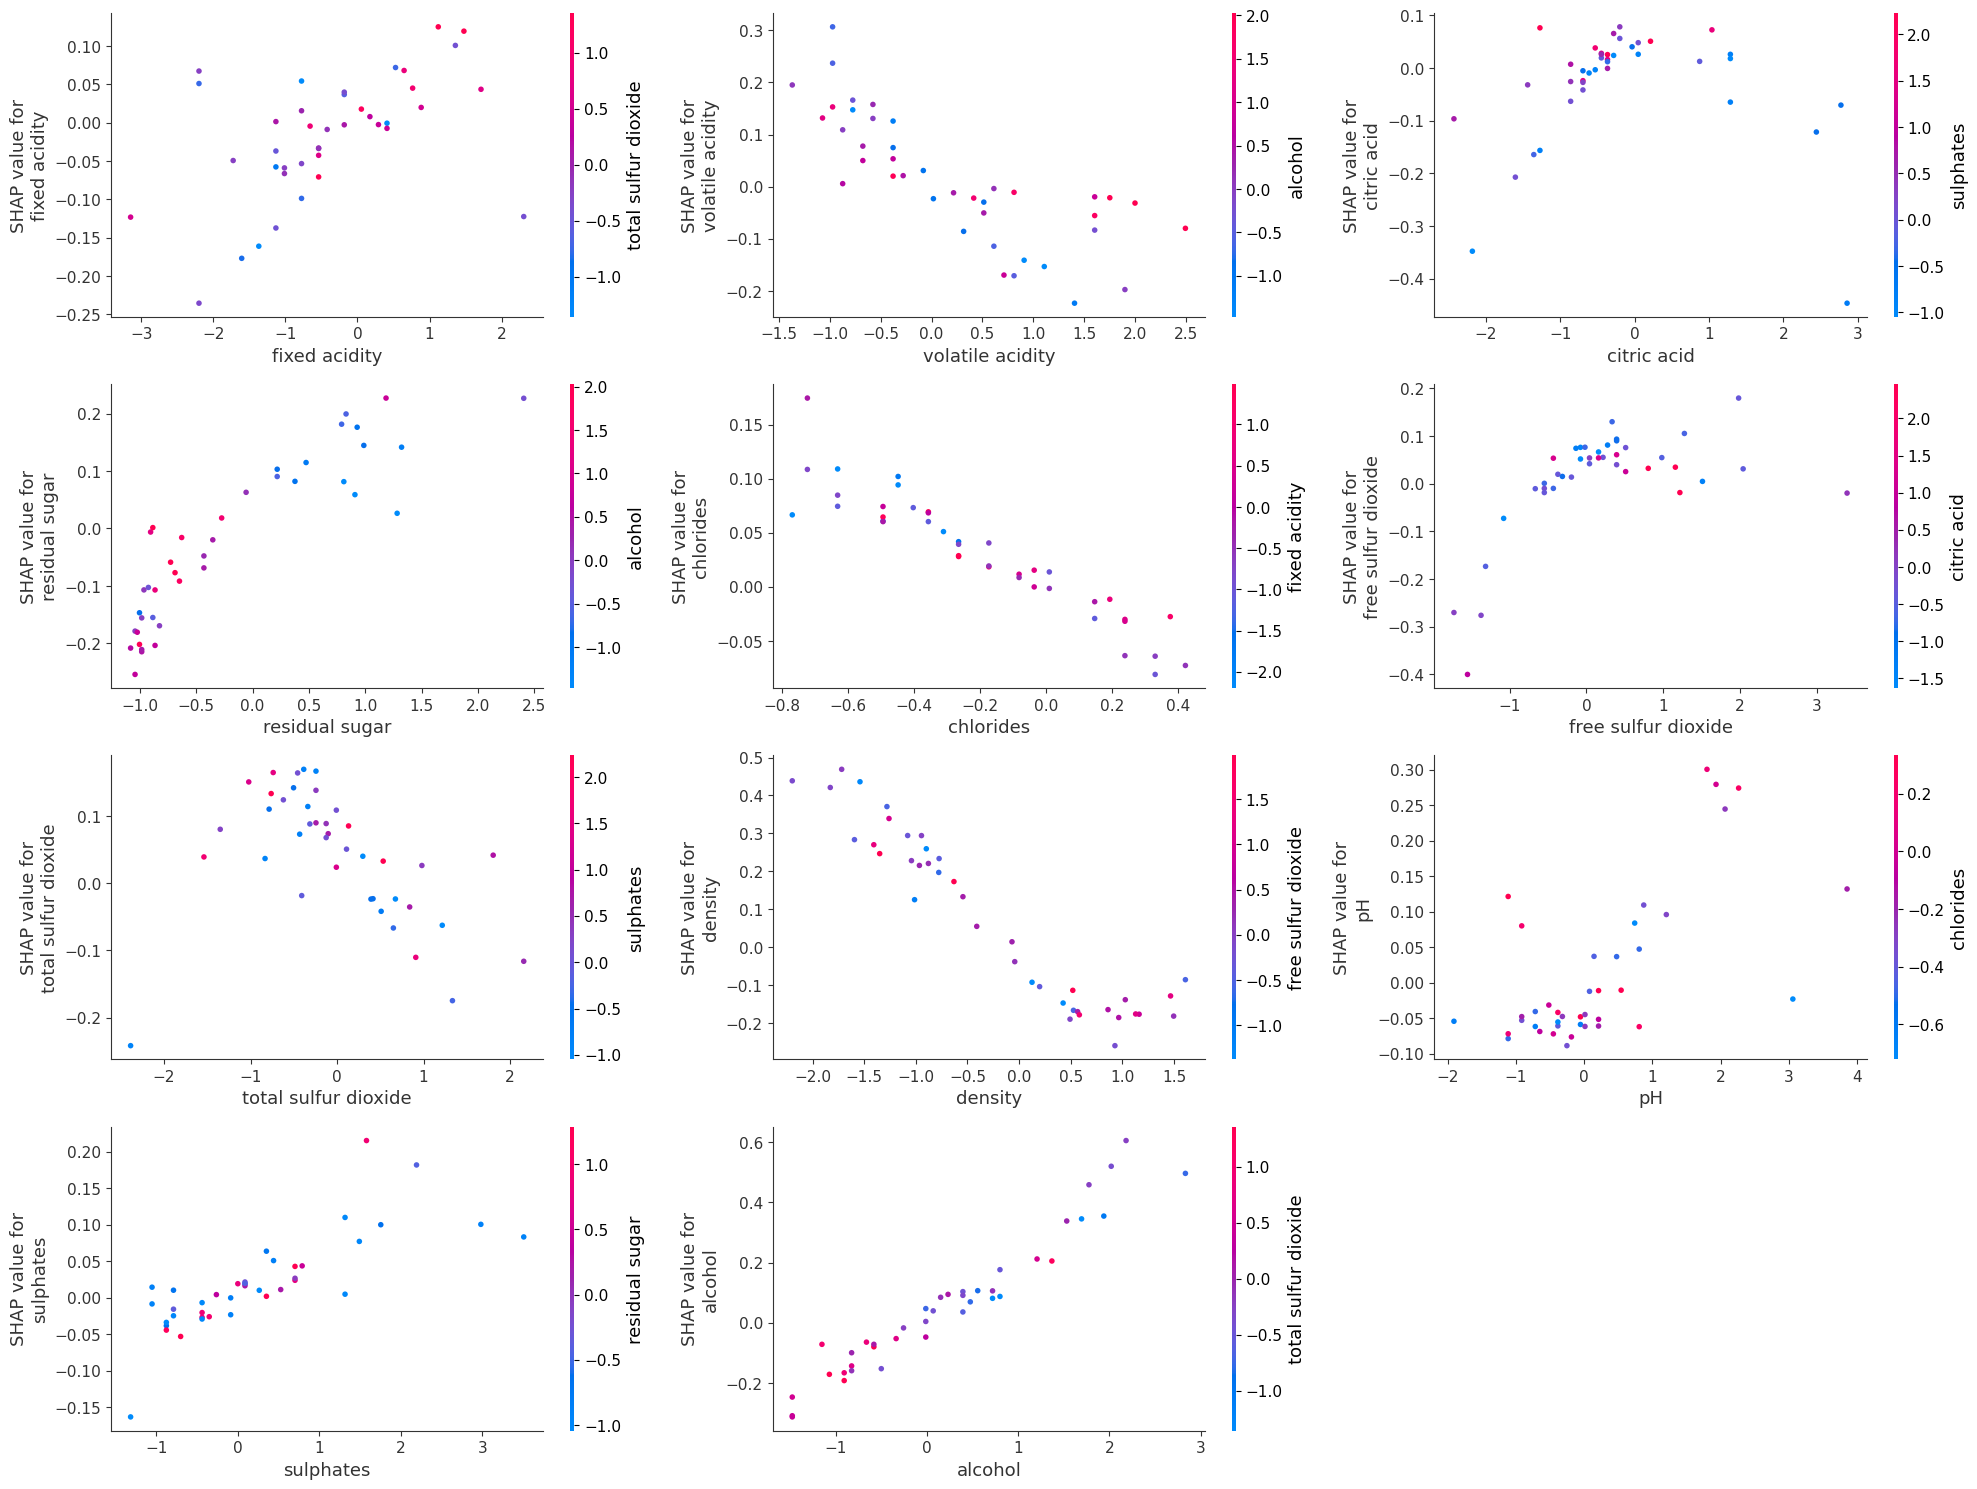
\includegraphics[width=\linewidth]{figures/shap-dependency-svr.png}
    \caption{Dependency plot of the features for SVR}
    \label{fig:dependency-plot-svr}
\end{figure*}
\subsubsubsection{Improve the model}
To optimize the model, the cost and gamma were examined. BayesSearch was used to find a model with the lowest possible mean squared error. 

\subsubsection{Results}

\subsubsubsection{Reproduce the results}
\begin{figure*}
\centering
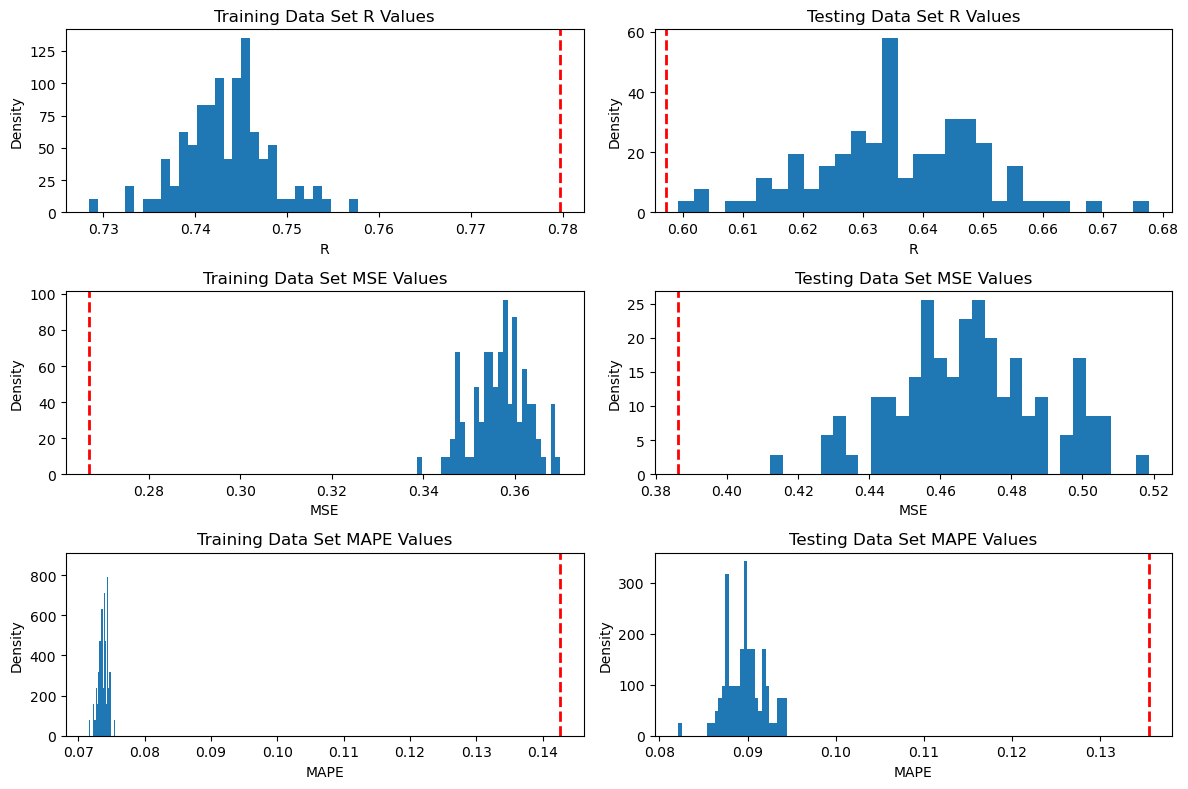
\includegraphics[width=\linewidth]{figures/SVR_reproduce_the_results.png}
\caption{Reproduce the results}
\label{fig:Reproduce-SVR-the-results}
\end{figure*}

\subsubsubsection{Impact of the features}
tbc


\subsubsubsection{Inprove the model}

In figure \ref{Reproduce-SVR-the-results} the best possible values for gamma and cost are examined. The non-optimized model (the model with the parameters as indicated in the article) is visualized by a blue sphere.
\begin{figure*}
    \centering
    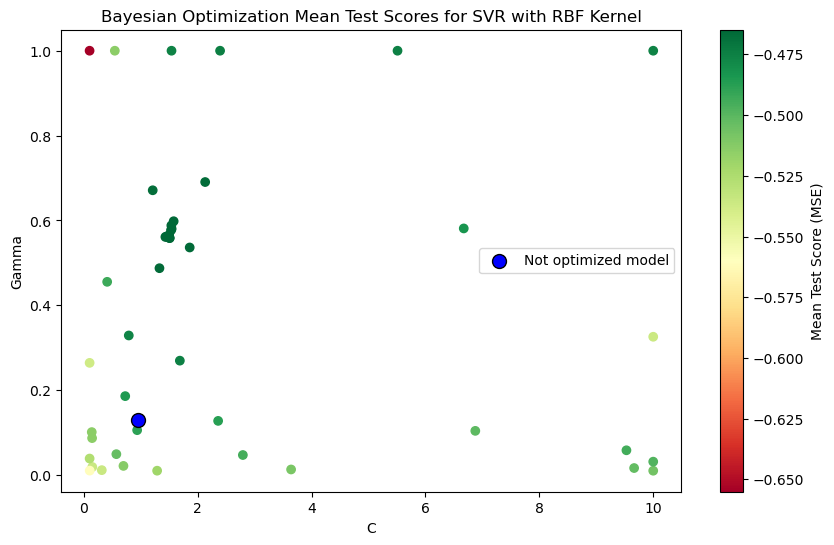
\includegraphics[width=\linewidth]{figures/bayesian_optimization.png}
    \caption{Bayesian search for optimal gamma en cost}
    \label{fig:optimized-model}
\end{figure*}

The most optimal parameters are: cost=1.51 and gamma=0.558.
In figure \ref{optimized-model} we see how the model performs compared to the values of the article model (dashed line) and compared to the non-optimized model (dotted line).
\begin{figure*}
	\centering
	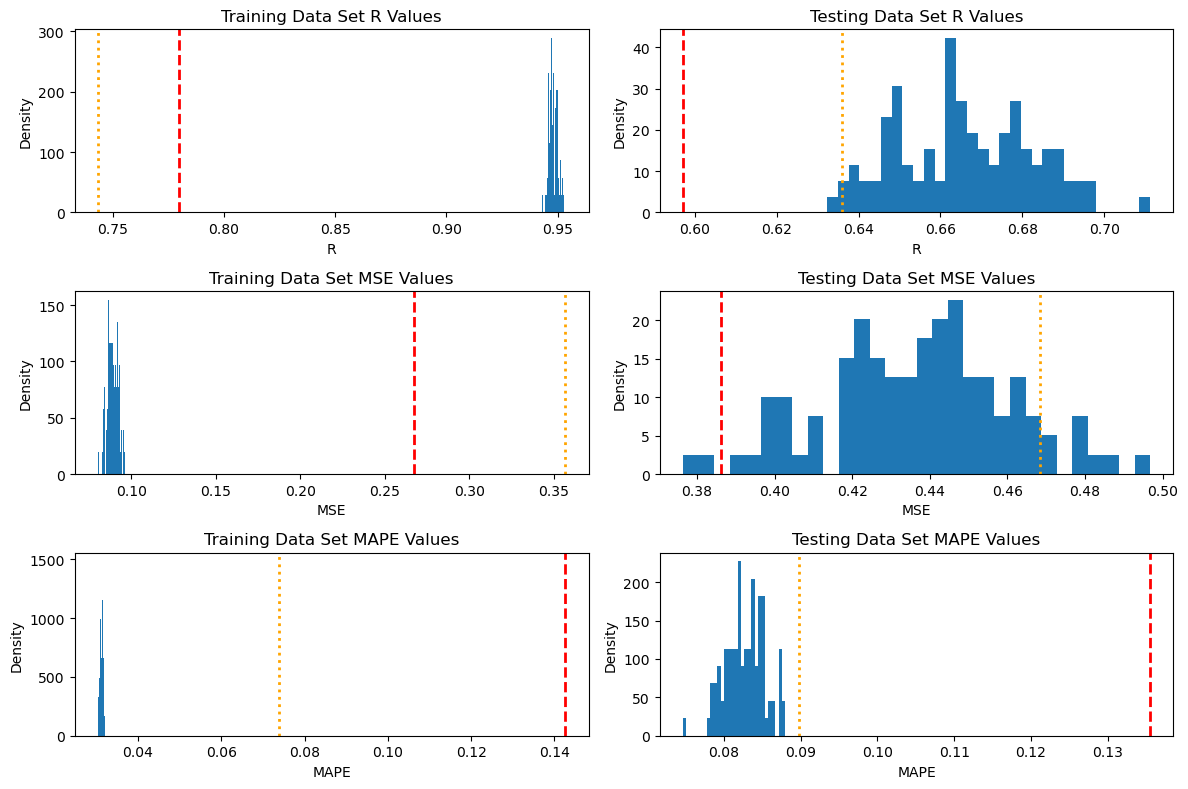
\includegraphics[width=\linewidth]{figures/SVR_optimized_model.png}
	\caption{Bayesian search for optimal gamma en cost}
	\label{fig:one-col-figure}
\end{figure*}


\subsubsection{Discussion}
%Additionally, you can include a separate discussion section in which you summarize the results, indicate possible limitations of your work, and provide suggestions for future research.


The results of the article have been reproduced. The impact of the features has been investigated. And the model has been optimized. All this while the article does not seem reliable because of the incorrect naming of the data set (namely red wine instead of white wine)


\subsection{Citing references}
LaTeX manages the citations for you. You simply have to add the bibtex entry for the reference in the references.bib file and you can use the citation in the paper \cite{langley00}. You can also cite multiple references in one command \cite{DudaHart2nd,Newell81,kearns89}. The bibtex entries for a paper can be obtained in websites such as google scholar or dblp.

\subsection{ANN}

\subsubsection{Datasets}
In the article it is stated that the train-validation-test ratio is 60-20-20. We have also maintained this ratio for reproducing and optimizing the model.

\subsubsection{Implementation Details}

\subsubsubsection{Reproduce the results}
The article mentions the following parameters: 1 input layer, 3 hidden layers (each with 15 neurons) and one output layer with the Adam optimizer.
As activation function relu was chosen and the mean squared error as loss to optimize.
How the training data is chosen is unknown, so the split between training and test data is performed multiple times. In this way, there is a realistic picture of the models that generate these parameters.

\subsubsubsection{Impact of the features}
tbc

\subsubsubsection{Inprove the model}
Due to time constraints, we will limit the number of tests. Gridsearch will be used to see if the model can be optimized by adjusting the number of neurons in the hidden layers.
It was also considered to reduce the number of hidden layers to one. The reasoning behind this is that the data is not that complex and that the complexity of the three layers would be unnecessary. With one hidden layer, the impact of the number of neurons is also considered. And once an optimum has been found, the impact of batch size and epochs is also examined.

\subsubsection{Results}

\subsubsubsection{Reproduce the results}

In figure \ref{fig:ANN-reproduce-the-results} the original model is indicated by a red dashed line. With the chosen parameters 100 models were trained and shown as blue bar charts. The average of the bar charts is shown by an orange dotted line.
The R values are very similar. The MSE results are worse than those of the model from the article while the MAPE results are better than those from the article.
The combination of a higher MSE and a lower MAPE may indicate that most forecasts are accurate, but there are some exceptions with large errors that increase the MSE.
This must be put into perspective, because we are talking about very small differences compared to the original model. If we know that the quality has no significant figures, the differences compared to the original model are negligible.


\subsubsubsection{Impact of the features}
tbc

\subsubsubsection{Inprove the model}
Based on figure \ref{ANN-impact-neurons-3layers} it can be concluded that the model with 15 neurons for each layer is quite well chosen. Increasing the number of neurons will certainly not give better results.
With one neuron the story is different, see figure \ref{ANN-impact-neurons-1layer}. The model improves as the number of neurons increases with a flattening starting around 70 neurons. With these 70 neurons the impact of batch size and epochs was investigated with the aim of finding a better model.
As expected we see that we get better models at higher epochs and smaller batch sizes. For the final model epochs = 40 and batch size = 16 were chosen.

Figure \ref{fig:ANN-optimized-model} shows the model from the article with a red dashed line and the reproduced model with an orange dotted line. The blue bars show an optimized model with one layer (with 70 neurons). Both the R values, MSE and MAPE give better results than the reproduced model. This improvement is only minimal.


\begin{figure*}
	\centering
	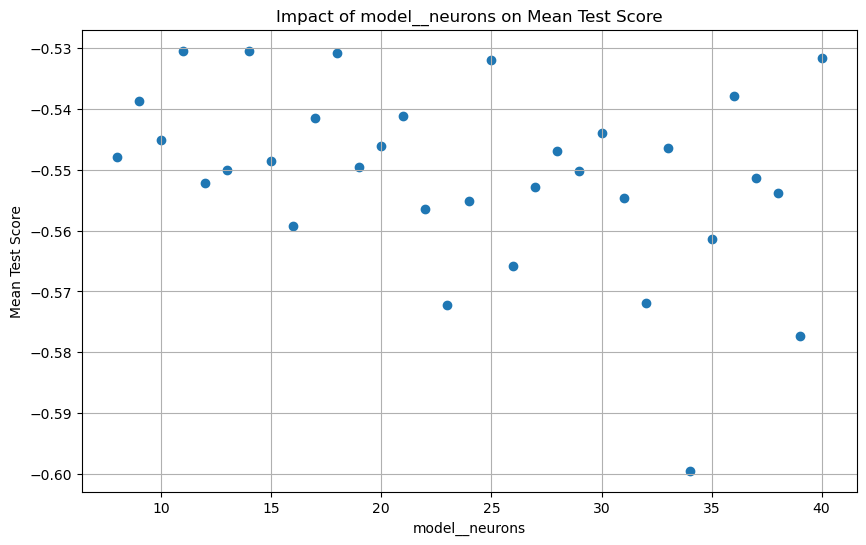
\includegraphics[width=\linewidth]{figures/ANN_impact_neurons_3layers.png}
	\caption{ANN impact neurons 3layers}
	\label{fig:ANN-impact-neurons-3layers}
\end{figure*}

\begin{figure*}
	\centering
	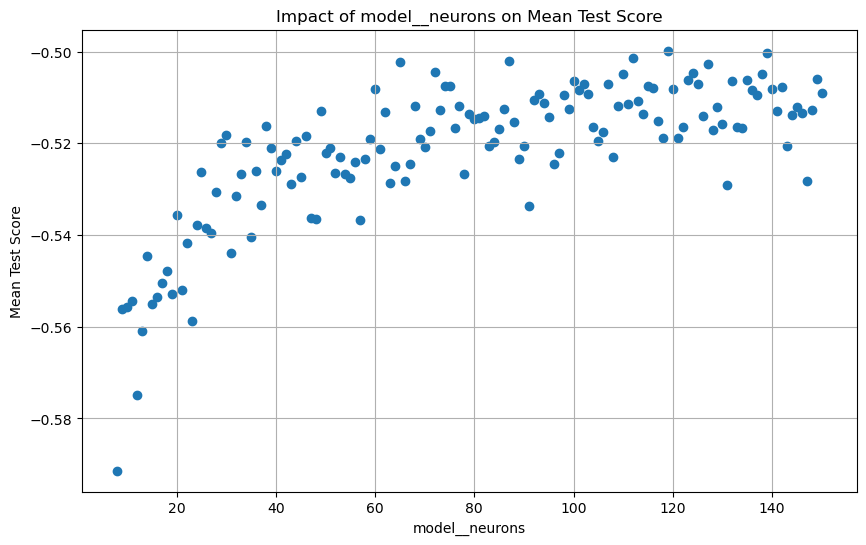
\includegraphics[width=\linewidth]{figures/ANN_impact_neurons_1layer.png}
	\caption{ANN impact neurons 1layer}
	\label{fig:ANN-impact-neurons-1layer}
\end{figure*}

\begin{figure*}
	\centering
	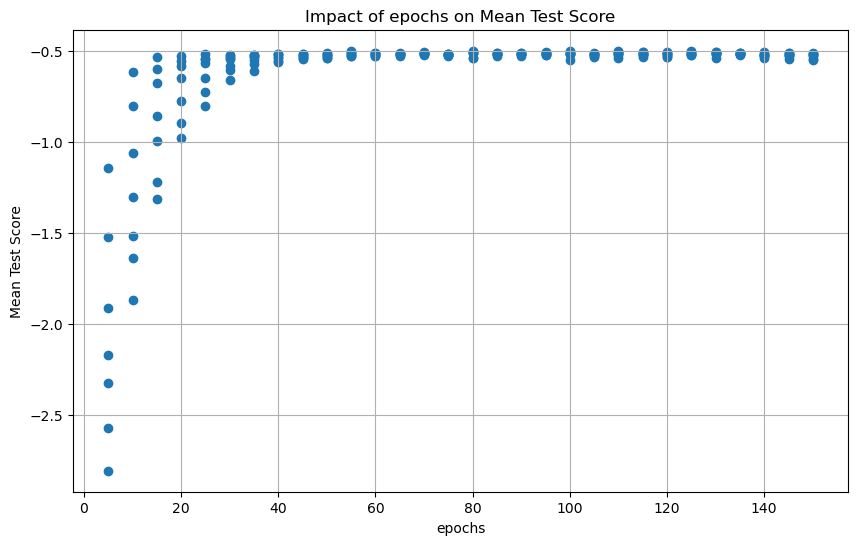
\includegraphics[width=\linewidth]{figures/ANN_impact_epochs_1layer.png}
	\caption{ANN impact epochs 1layer}
	\label{fig:ANN-impact-epochs-1layer}
\end{figure*}

\begin{figure*}
	\centering
	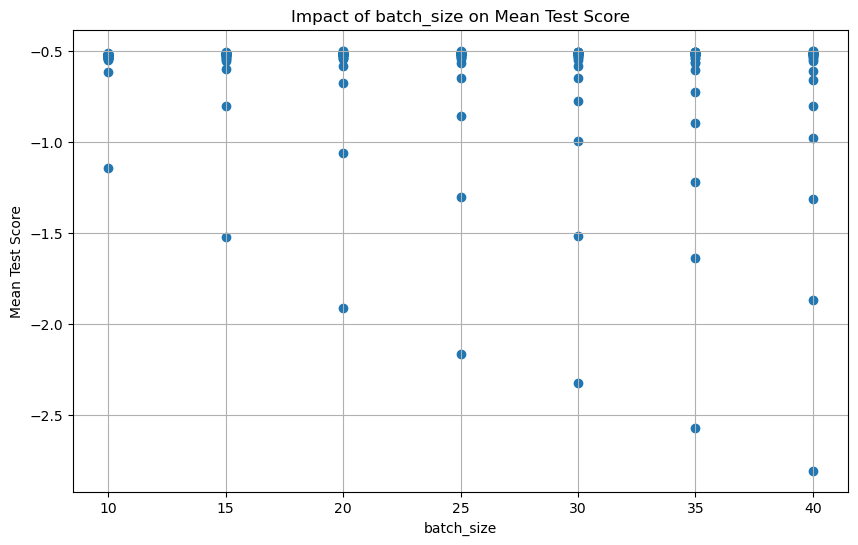
\includegraphics[width=\linewidth]{figures/ANN_impact_batchsize_1layer.png}
	\caption{ANN impact batch size 1layer}
	\label{fig:ANN-impact-batchsize-1layer}
\end{figure*}

\begin{figure*}
	\centering
	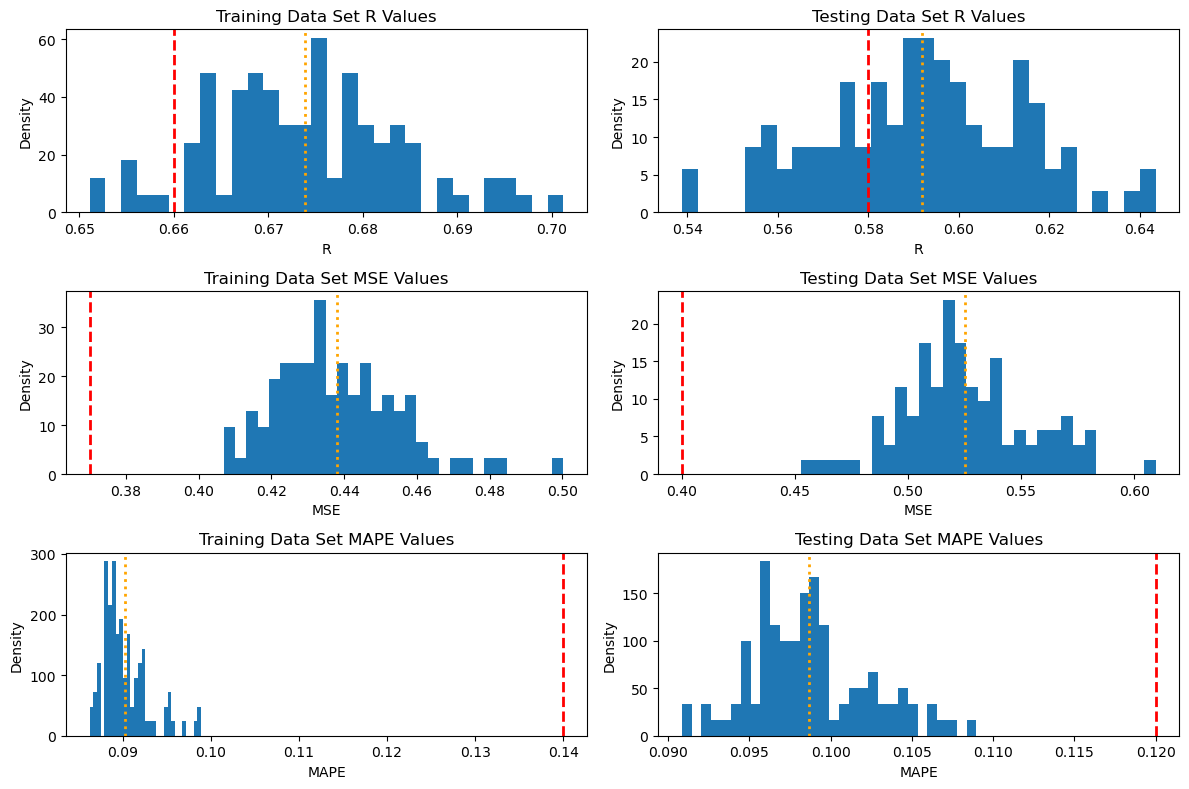
\includegraphics[width=\linewidth]{figures/ANN_reproduce_the_results.png}
	\caption{ANN: reproduce the results}
	\label{fig:ANN-reproduce-the-results}
\end{figure*}

\begin{figure*}
	\centering
	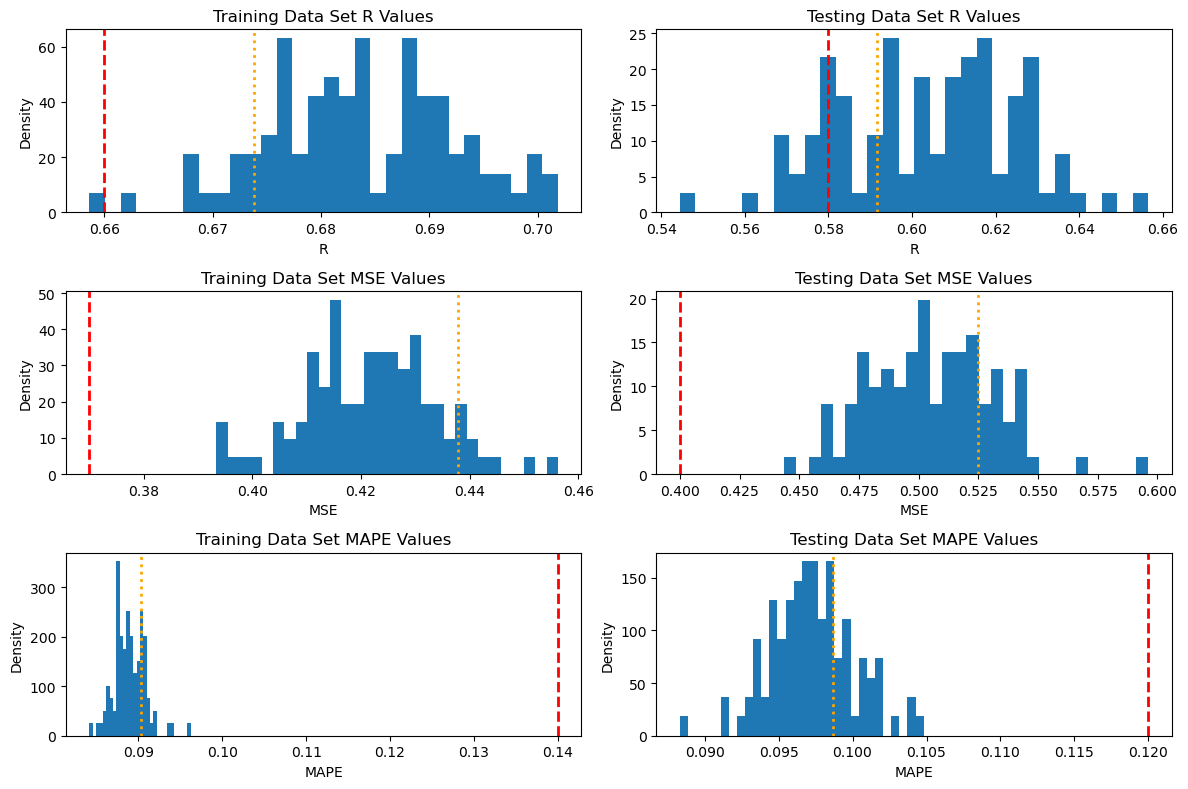
\includegraphics[width=\linewidth]{figures/ANN_optimized_model.png}
	\caption{ANN optimized model}
	\label{fig:ANN-optimized-model}
\end{figure*}




\subsubsection{Discussion}




\subsubsection{Citing references}


\bibliography{references}
\bibliographystyle{icml2021}


\end{document}

